\scanpage{33}
\uline{Prop} Autre caractérisation de $\operatorname{Fr}_{F/X}^*$ pour $X$ fixé : c'est un hom fonctoriel en $F$, et pour $F$ \uline{représentable} \inserted{par $X'$ étale$/X$} c'est l'hom de Frobénius habituel noté $\operatorname{Fr}_{X'/X}$.
\margin{\figure{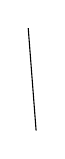
\begin{tikzpicture}\draw (0,0)--(.1,-1.3);\end{tikzpicture}}}

\uline{Théorème de trivialité cohomologique du Frobénius absolu.}
L'hom
\diagram{\begin{tikzcd}[column sep=large,row sep=large]
H^0(X,F) \arrow[d,phantom,"\wr" description] & H^0(X,F)\\
H^0(X,\operatorname{Fr}_{X*}(F)) \arrow[ur,"H^0(\operatorname{Fr}_{F/X})"'] &
\arrow[from=1-1,to=1-2,phantom,"\deleted{\unsure{\longrightarrow}}" description]
\end{tikzcd}}
est l'\uline{identité}, pour $\forall$ faisceau $F$ sur $X_{\text{ét.}}$.
\margin{\figure{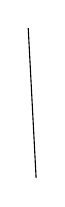
\begin{tikzpicture}\draw (0,0)--(.1,-1.9);\end{tikzpicture}}}

\uline{Corollaire} 1 Si $F$ est un faisceau en groupes,
\diagram{\begin{tikzcd}[column sep=large,row sep=large]
H^1(X,F) \arrow[d,phantom,"\wr" description] & H^1(X,F)\\
H^1(X,\operatorname{Fr}_{X*}(F)) \arrow[ur,"H^1(\operatorname{Fr}_{F/X})"'] &
\end{tikzcd}}
est l'\uline{identité}.

\uline{Corollaire} 2 Si $F^\bullet$ est un \inserted{complexe de} faisceaux \deleted{\unsure{abéliens, des}} \inserted{de $A$-Modules} ($A$ un \deleted{faisceau \unsure{d'anneaux}} \inserted{anneau quelconque}) \inserted{$F^\bullet$ borné sup.}, alors
\diagram{\begin{tikzcd}[column sep=large,row sep=large]
\mathrm R\Gamma_X(F^\bullet) \arrow[d,phantom,"\wr" description] & \mathrm R\Gamma_X(F)\\
\mathrm R\Gamma_X(\operatorname{Fr}_{F^\bullet/X*}(F^\bullet)) \arrow[ur,"\mathrm R\Gamma_X(\operatorname{Fr}_{F^\bullet/X})"'] &
\arrow[from=1-1,to=1-2,phantom,"\deleted{\unsure{\longrightarrow}}" description]
\end{tikzcd}}
est l'\uline{identité} dans la catégorie \inserted{$D(A)$} dérivée de la catégorie des $A$-modules.
En particulier $H^i(X,F)\unsure{\mathbin{-}}H^i(X,F)$ est l'identité.

Ces corollaires résultent du th. en utilisant le calcul de $\mathrm R^1\Gamma_X$ resp. de $\mathrm R\Gamma_X$ par \uline{résolutions}. / Pour prouver le Thm, on note que \deleted{\unsure{si $s$ est une section}} \deleted{\unsure{on conclut par fonctorialité}} l'hom
\diagram{\begin{tikzcd}H^0(X,F) \arrow[r,no head,"H^0(\operatorname{Fr}_{F/X})"] & H^0(X,F)\end{tikzcd}}
est \uline{fonctoriel} en $F$. D'autre part, si $F$ est le faisceau final, c'est l'identité, grâce à la prop. Ces deux faits ensemble donnent \unsure{trivialt} la conclusion.
\mspage{32}
